\TODO{L: I need to spelcheck at some point}
\TODO{L: Regenerate the renders}
%%%%%%%%%%%%%%%%%%%%%%%%%%%%%%%%%%%%%%%%%%%%%%%%%%%%%%%%%%%%%%%%%%%%%

\section{Introduction}
\label{sec:intro}


Raytracing is a foundational technique in computer graphics, which can be used
to render photorealistic scenes.
A good introduction to the main techniques and practical implementations can be found
in Ref.\cite{raytracing_in_one_weekend}.
In general this implies expensive processes and requires the corresponding appropriate compute time
as well as complex and sophisticated algorithms.
Their applications \cite{Peddie2019_appns} range from generation of high-quality realistic visualizations to
rendering of movies or animations, and up to even more exotic images of black holes,
such as the ones remarkably done for the black hole residing at the center of the galaxy M87 \cite{M87_EHT_i}
and the supermassive black hole Sagittarius A* at the center of our own galaxy \cite{SagA_EHT_i}.
In these cases, ray-tracing techniques have been applied to
General Relativistic Magneto-HydroDynamics simulations in order to produce 
the so-called fiducial templated models of the event horizon images.
These techniques have allowed us to produce images that have captivated the minds and interest of millions.
After establishing the theory and equations for describing the trajectories of light rays around a black hole, it is natural to try to use a ray tracer to render a scene within this geometry which ultimately results in a particular distortion applied to the general techniques.

We should emphasize that there exist a large variety of ray tracer implementations already 
\cite{imbens2023graphicalprocessinggeodesicpropagation,10.2312/EGPGV/EGPGV12/051-060,7539599_OSPRay}
and even ones with direct astrophysical applications such as the rendering of black hole surroundings
\cite{10.2312:vmv.20221208,sharma2023mahakalapythonbasedmodularraytracing,James_2015}.
However, our approach seeks to highlight some specific features:
i) its open-source implementation;
ii) the minimalistic and simplistic implementation strategy, i.e. by tackling
mostly the actual mathematical problem using specialized libraries
to solve the governing differential equation of the problem;
iii) the ease of implementation in a fairly efficient and high-performing
way by employing standards in shared-memory and distributed-memory paradigms;
and iv) the hardware agnostic approach, i.e. not depending on specialized hardware, accelerators or GPUs \cite{Peddie2019_hardware}
which one could argue would be better suited for tackling this type of problems.

In order to model a simple black hole scenario, we can use the Schwarzschild metric \cite{schw_soln-2007}.
This models black holes which, among other properties, are non-spinning and not charged,
meaning that their deformation of the trajectories of light rays do not depend on the angle of approach.
It has been well established \cite{gravitation-mtw} that the equation,
\begin{equation}
	u'' - u = 3 M u^2
	\label{eq:Sch-light-ray}
\end{equation}
relates the trajectory of a light ray to the mass $M$ of a black hole, from the Schwarzschild metric;
where $u$ represents $1/r$, $r$ being the Euclidean distance of a point on the light ray to the black hole center.
$u$ is differentiated with respect to $\phi$, the azimuthal angle between the point and the black hole origin.
See Fig.~\ref{fig:nextpoint} and its accompanying section for more detail on the geometry of this equation.
After providing initial conditions,  it is possible to solve Eq.(\ref{eq:Sch-light-ray}) and trace the entire trajectory of the ray with high fidelity.
Notably, this equation is modeled in 2D-spherical coordinates, meaning, if we want to use this equation to analyze light rays in 3D space, we need to find a way to find an equivalent ray that our equation models, and use the 2D ray to find the 3D ray's trajectory.

After being able to compute the trajectory of individual rays, we can use these rays to generate a full image using ray tracing. Ray tracers render a simulated scene by casting light rays from a simulated camera, and computing what objects in the scene would be visible to that ray. Hypothetically, if a particular camera would produce an image of $1920 \times 1080$ pixels, we could build the image that camera would record by casting a light ray through each pixel. Because ray tracing's unit of perception is how simulated light rays interact with a simulated scene, it is a natural choice for simulations which involve the bending or distortion of light.

%NOTE: Liam: I don't like this section since it breaks up the flow of the previous paragraph to the next
%Having given an introduction in Sec.~\ref{sec:intro} to the problem, we will proceed in Sec.~\ref{sec:impl} to describe our implementation approach, followed by results in  Sec.~\ref{sec:results} and a discussion in Sec.~\ref{sec:disc} and ~\ref{sec:concl}.


%%%%%%%%%%%%%%%%%%%%%%%%%%%%%%%%%%%%%%%%%%%%%%%%%%%%%%%%%%%%%%%%%%%%%

\section{Implementation}
\label{sec:impl}


\subsection{Approximating the trajectory of a light ray as a piecewise function}
While the fundamental idea of taking a ray tracer and modifying it so that light rays are distorted is sound, the implementation of such an idea is fraught with difficulty. The first major challenge is that ray tracers need linear equations to be able to compute object intersection in a scene. This means we need to find a way to describe our light ray as a piecewise-defined set of linear equations. We found the best way to do this was to compute discrete points on the light ray, and compute intersection using the line segments defined by said points. 


\subsection{Using GSL for ODE approximation}
As for how to compute these segments, the GNU Scientific Library's (GSL) suite \cite{10.5555/1538674} of ODE approximation tools found significant utility. GSL allows us to define our equations as C functions, and our particular ray by a set of initial conditions. From there, we can use GSL to compute a series of discrete points on the ray governed by a timestep of our choosing. For initial conditions, we need to describe, in 2D spherical coordinates, an initial point on the ray and a single successor point, which was computed using the linear direction, as we are casting rays far from the black hole's influence. As for the \textit{timestep} (as it is commonly known in the GSL documentation), we allowed program users to control the distance between computed points, which we will refer to as $\varepsilon$, i.e. the \textit{discretization} or \textit{step} of the simulation. Lower values of $\varepsilon$ result in more accurate trajectories, but also require more computed points. 

\subsection{Ensuring even spacing of computed points}
To compute the next point on a light ray $\varepsilon$ distance away, we would compute, using the Euclidean metric, the light ray's path with no distortion. In spherical coordinates, this allows us to compute the azimuthal angle from the black hole's origin. We can feed this updated azimuthal angle into GSL, and it will return the distance of the ray from the origin of the black hole. In effect, GSL behaves as a function from azimuthal angle to distance, allowing us to compute the needed points in 2D space.
Fig~\ref{fig:nextpoint} despites an example of how these paths are computed.

\begin{figure}[h]
  \centering
  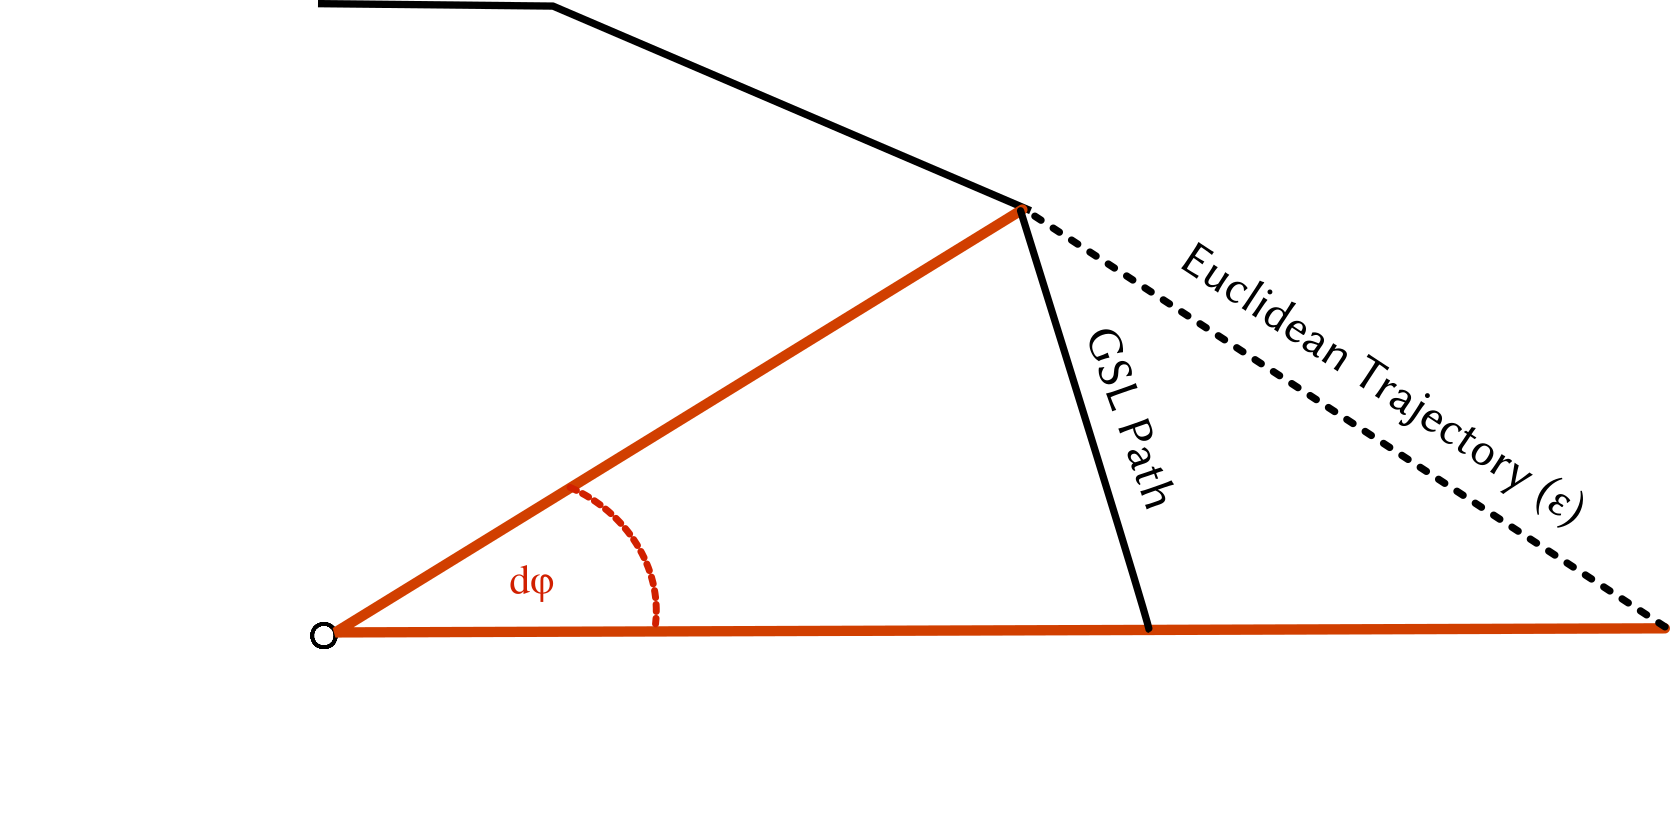
\includegraphics[width=.65\linewidth]{figs/nextpoint}
  \caption{We use Euclidean geometry to compute $d\phi$, then rely on GSL to stencil the ray's path until the simulation progresses by $d\phi$}
  \label{fig:nextpoint}
\end{figure}


\subsection{Relating our 2-variable equation to 3D space.}
As noted earlier though, we cannot use the trajectories of rays in 2D space to render a 3D scene, meaning we need to find a way to find a 1-to-1 relationship between a subset of 3D rays and 2D rays. The solution here was to recognize that we could apply a combination of axis rotations and axis relabeling to complete the correlation. If the "origin" of the light ray, and the origin of the black hole are both located on the z axis, as is the case for our 3D scenes, we can rotate our ray around the z axis until the ray's direction vector has incline $ \pi / 2 $ with respect to the black hole origin, meaning the ray has no spherical incline. At this point, the y component of the ray's origin and direction will both be zero, meaning we have reduced our 3D ray to 2D. From here, we can easily convert to spherical coordinates for use with GSL. Since this process is invertible, we have now found a way to use GSL to trace the trajectory of light rays in 3D using an equation of two variables.


\subsection{Image and scene handling}
%https://scholar.google.com/scholar?hl=en&as_sdt=0%2C5&q=boost+GIL+Generic+Image+Library&btnG=
Image and scene handling was done both with JPEG and with PPM support.
For JPEG support, the Boost's Generic Image Library
\cite{schaling_boost,bourdev2007generic} (and consequently libjpeg) was used, and for PPM support, a custom parser was written. Both of these parsers rely on loading the entire image into memory, which has the advantage of quick pixel access, at the cost of potentially loading a lot of unused pixel data into memory. For moderately sized images, this is an appropriate tradeoff, however, for very large astronomical images, this could quickly become a problem, especially as the size of an image (Plus whatever memory is needed for rendering) eclipses the available RAM. To deal with this, future implementations could apply a number of techniques:
1. Refuse to load the image into memory, instead relying on an `fseek+fread` style implementation, which is likely to perform well on SSD storage, but poorly over the network.
2. Decompose the image, and have each process store a portion in memory, at the cost of having to exchange pixels when a light ray "misses" our portion of the image. This strategy, if poorly optimized, could result in horrible performance, as it's quite difficult to predict the trajectories of an arbitrary light ray in advance, meaning we are likely to miss our loaded portion of the image. This could easily yield a network bottleneck.
3. Load portions of the image that are relevant to our render only. This is somewhat of a balance of the previous two approaches, at the cost of additional complexity. 


\subsection{Domain Decomposition}
The essential element of speeding up a problem with Message Passing Interface (MPI) \cite{mpi41} is often to attempt to decompose the problem space into subproblems which can be computed on an individual node. In our case, our problem space is the image we are attempting to render. The most simple solution is to decompose along the scanlines, and render distinct scanlines on distinct nodes. In effect, one would attempt to assign a "band" to each process to render against. As a note, care must be taken to make sure that each process gets a relatively even number of rows, as if one simply divides the number of rows by the number of cores, and assigns it to each process, you are often left with a large remainder assigned to a single process that significantly slows down the speed of computation.

The downside of domain decomposition is that we now have separate bands rendered on separate processes. There are two potential variant implementations. One is to have the "child" processes send their rendered data to a single "parent"/"root" node, which outputs a single image. This is quite convenient for testing, as there is no work required to reassemble the image after rendering. The downside of this is that sending uncompressed pixel data across the network could be quite slow if one is rendering a large scene. To fix this, one could have each process write its "band" to a file, and recombine the images into a large scene later. If image output is done in PPM, this recombination is quite simple, and could likely even be done by a couple clever invocations of `cat`, `head`, and `tail`.


\subsection{Use of OpenMP}
In the context of a single band, it is quite easy to use OpenMP \cite{660313_OMP} to accelerate rendering, as the problem can be decomposed along the individual scanlines. This was quite helpful, as MPI was best used to distribute the problem across nodes, and OpenMP was useful for distributing the problem across cores.
Additionally, as shown in Sec.~\ref{sec:results}, OpenMP threads scale significantly better than MPI processes, meaning we would like to take advantage of the increased performance wherever possible.


\subsection{Code Availability}
Based on all the elements described in the previous sections,
we developed our source code in C++ which is available in the following
GitHub repository:
	\url{https://github.com/liamnaddell/BHRaytracer}


%%%%%%%%%%%%%%%%%%%%%%%%%%%%%%%%%%%%%%%%%%%%%%%%%%%%%%%%%%%%%%%%%%%%%


\section{Results}
\label{sec:results}

\subsection{A selection of renders}

This section includes results of images rendered employing our ray tracer's implementation.
The background images for these renders were taken from NASA's Scientific Visualization Studio (\url{https://svs.gsfc.nasa.gov/}).
We present two images -- Figs.~\ref{fig:eagle} and \ref{fig:starry}, it is easy to see the effects of gravitational lensing, as well as the clear Einstein ring. 


\begin{figure}[h]
  \centering
  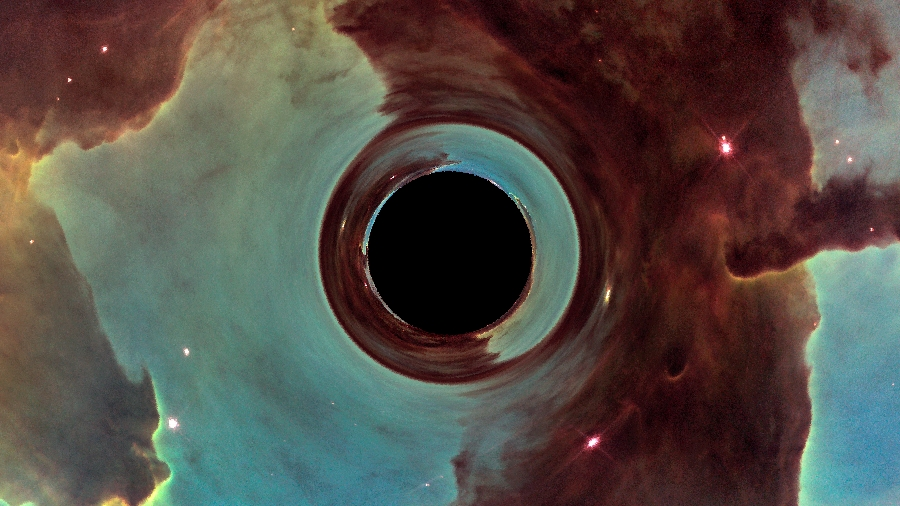
\includegraphics[width=0.8\linewidth]{figs/eagle_render}
  \caption{Image generated from a portion of the Eagle Nebula M16 downloaded from \cite{esa-pillars}.}
  \label{fig:eagle}
\end{figure}


\begin{figure}[h]
  \centering
  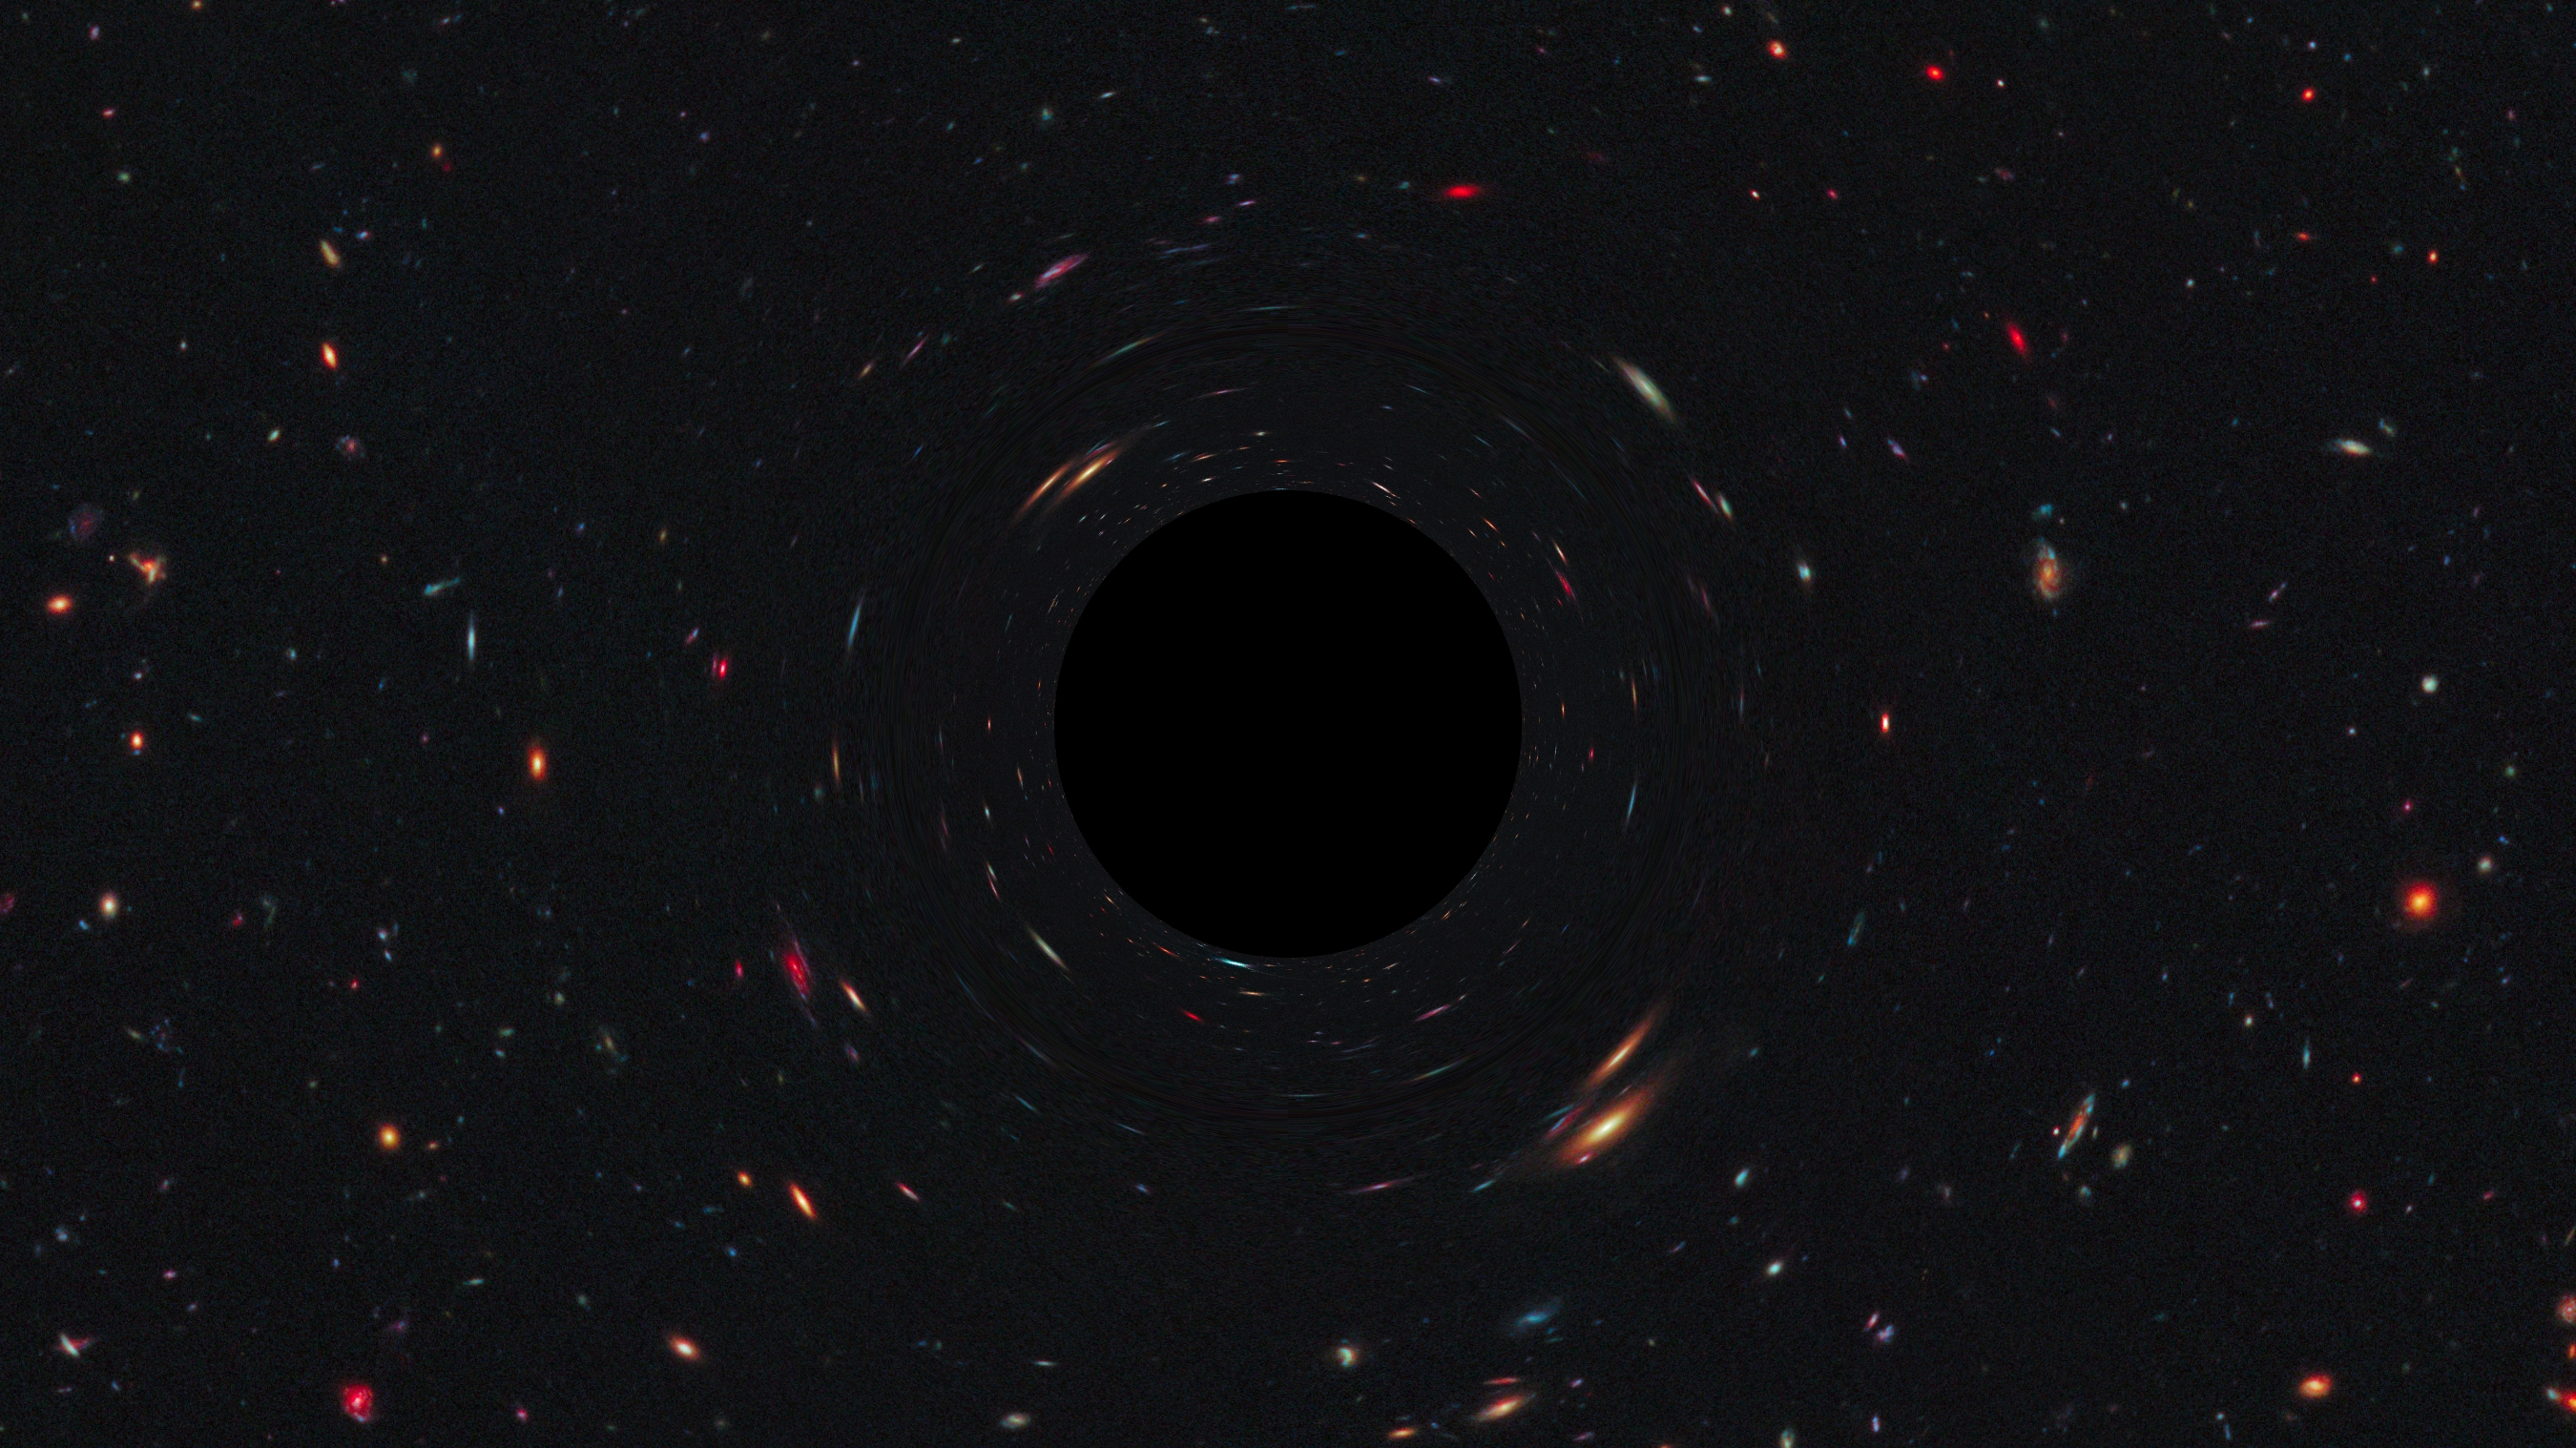
\includegraphics[width=0.8\linewidth]{figs/starry_render}
  \caption{A second example of an application from our ray tracer implementation,
	in this case from a deep star map from \cite{deepstarmap-nasa_svs}.
	The original image was edited just to raise its exposure.}
  \label{fig:starry}
\end{figure}




\subsection{Scaling analysis}

With this project, one can attempt to scale along many different axes. You can increase the size of the background image to stress image parsing, you can increase the number of rendered pixels, you can decrease $\varepsilon$, yielding to more calls into GSL, or you can increase samples-per-pixel which controls antialiasing. For weak scaling, you can also scale by adding more nodes, or by adding more cores. 

When increasing the size of the background image, this increases the time spent outside the parallel region, as the background image has to be parsed by each process, which is likely to take the same amount of time per node. As such, it does not present significant interest for scaling analysis.

However, decreasing $\varepsilon$ is an interesting scaling parameter, as it is responsible for some of the fidelity of a rendered image. The challenge is that it is hard to be sure how decreasing/increasing $\varepsilon$ will impact the amount of time needed for a GSL call, which makes it an interesting parameter.

We believe though, that the main parameters of interest are number of rendered pixels, and the number of cores used (across both multiple nodes and single nodes). For testing this kind of scaling without increasing the number of pixels in the scene, antialiasing level could be turned up.

\begin{figure*}[h]
  \centering
 \begin{minipage}{0.45\linewidth}
  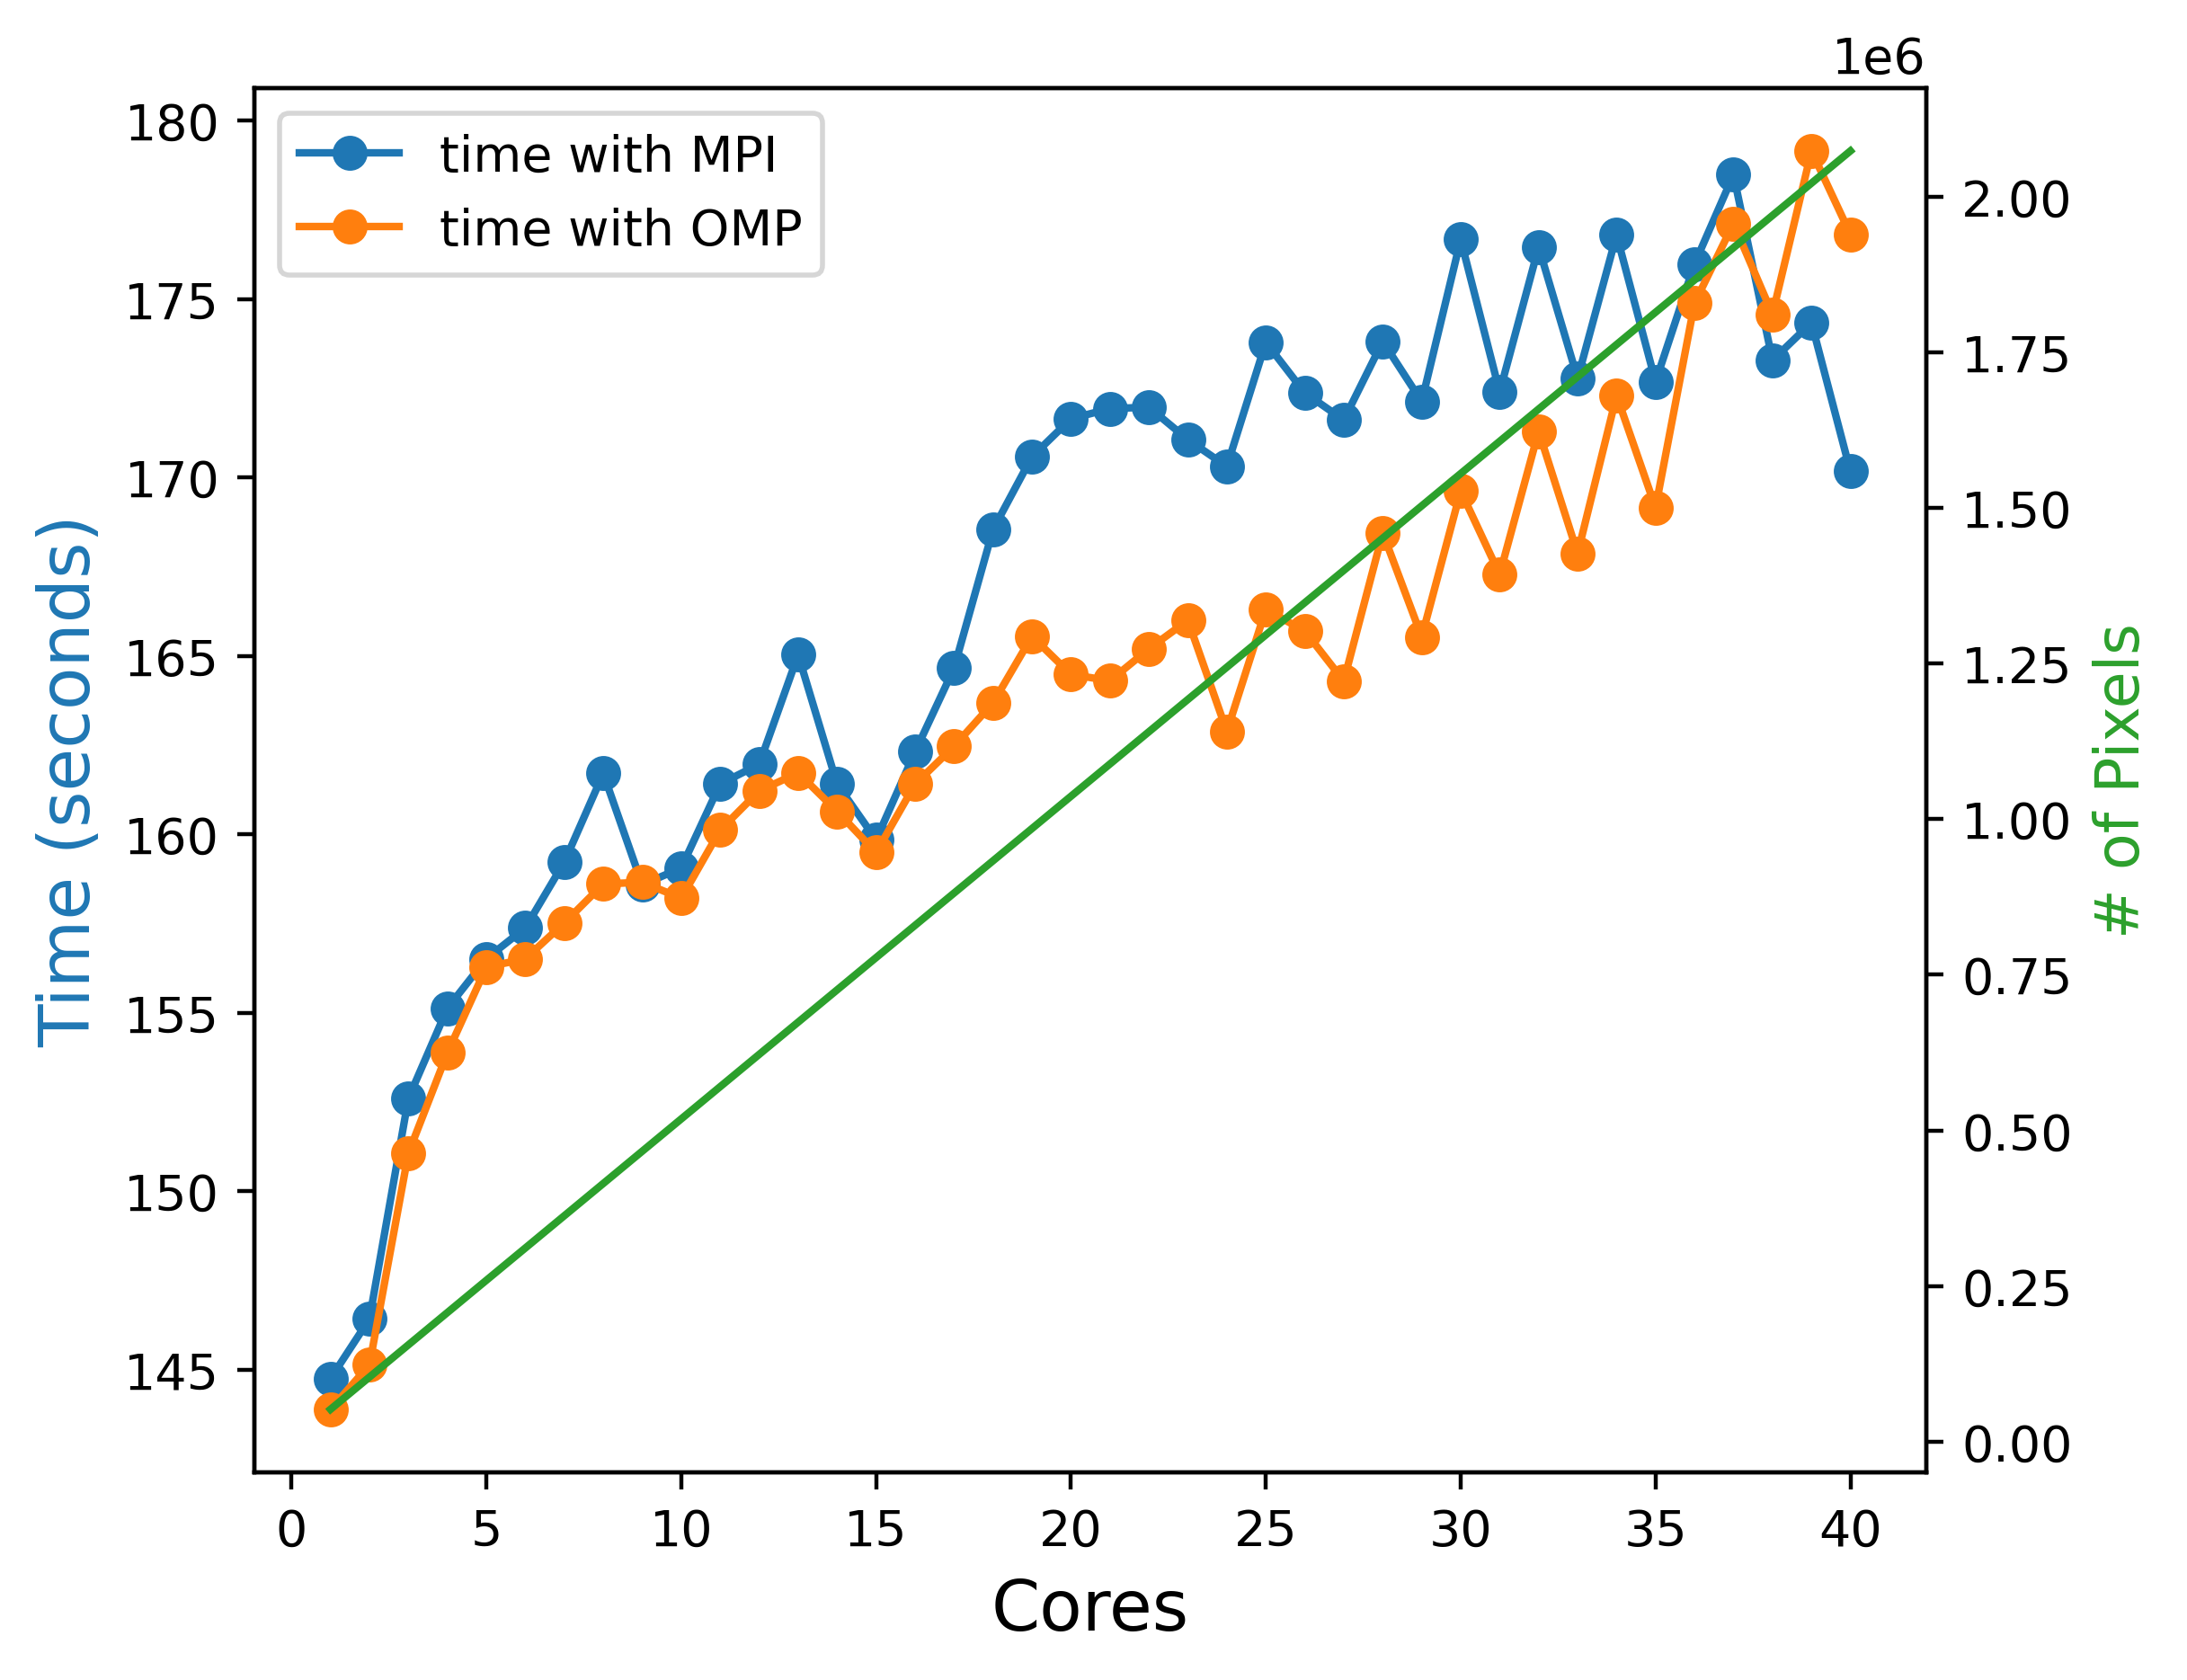
\includegraphics[width=\linewidth]{figs/mpi_weak2.out}
 \caption{Weak scaling analysis where MPI process count and image width are increased in tandem  }
	  \Description{As core count and image width increase linearly, time increases linearly }
    \label{fig:mpi_weak2}
    \end{minipage}
  \hspace{.05\linewidth}
  \begin{minipage}{0.45\linewidth}
      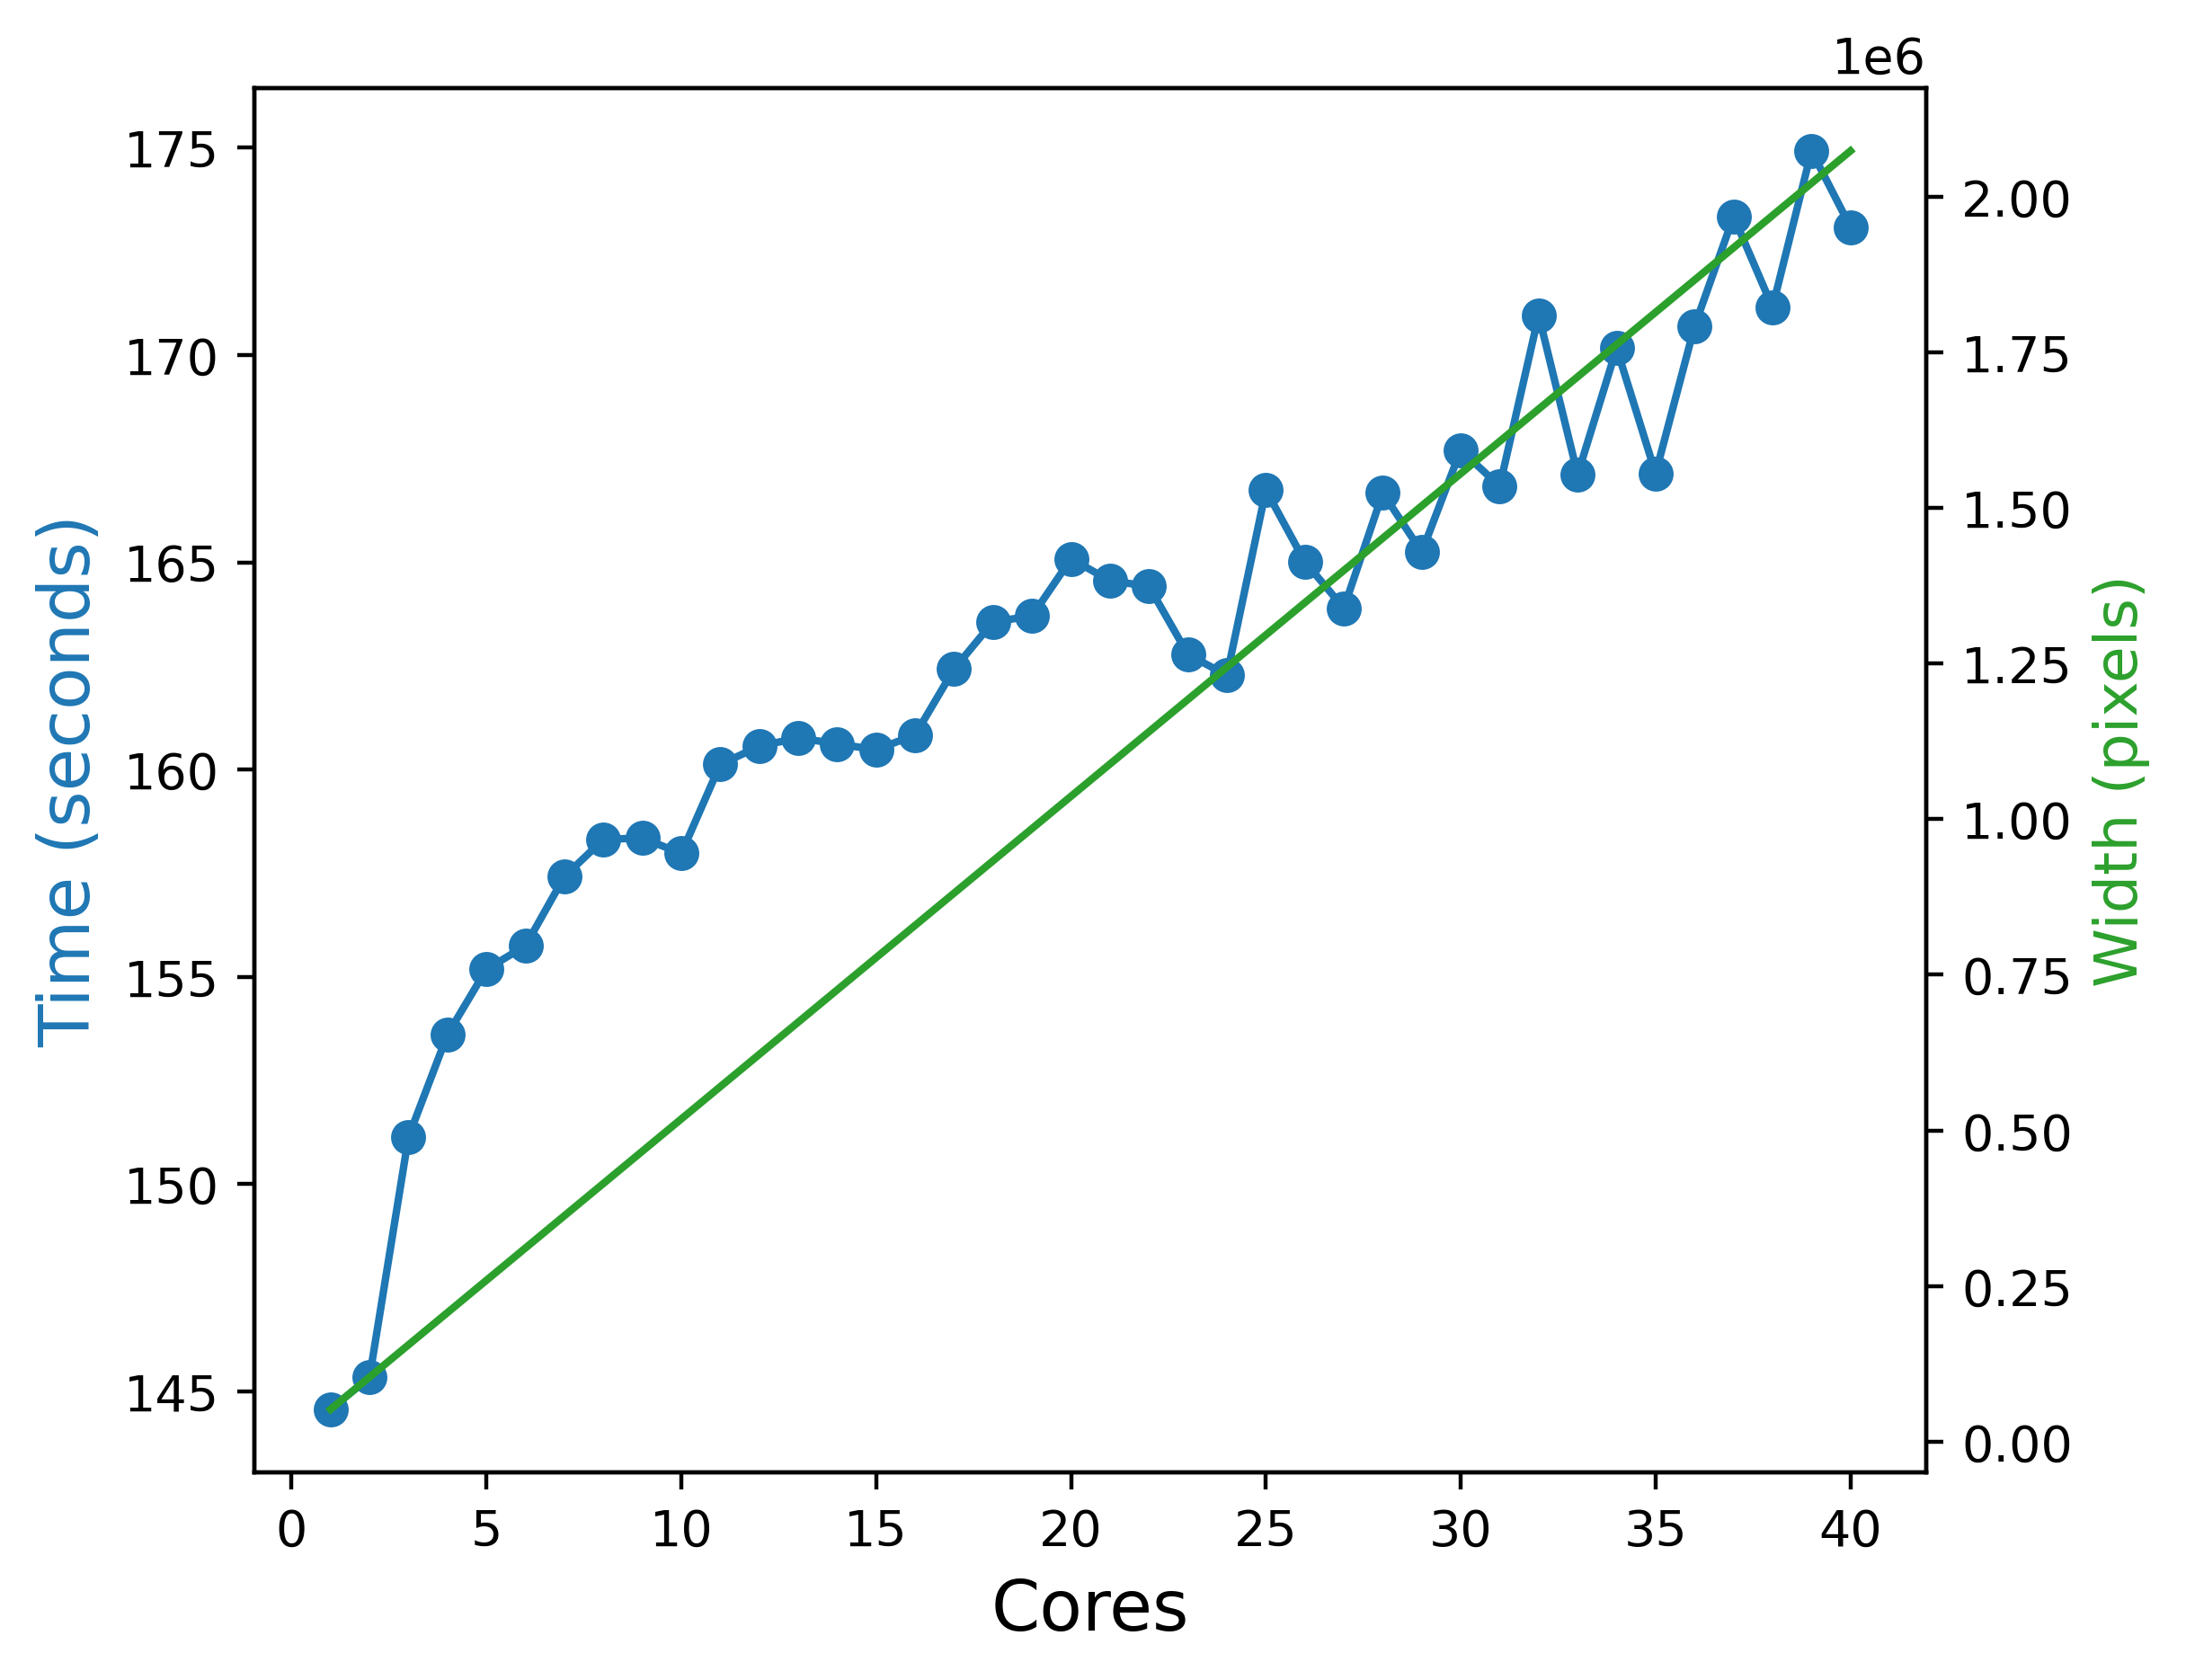
\includegraphics[width=\linewidth]{figs/omp_weak2.out}
      \caption{Weak scaling analysis where OMP threads utilized and image width are increased in tandem}
	  \Description{As core count and image width increase linearly, time increases linearly }
        \label{fig:omp_weak2}
    \end{minipage}
  \begin{minipage}{0.45\linewidth}
      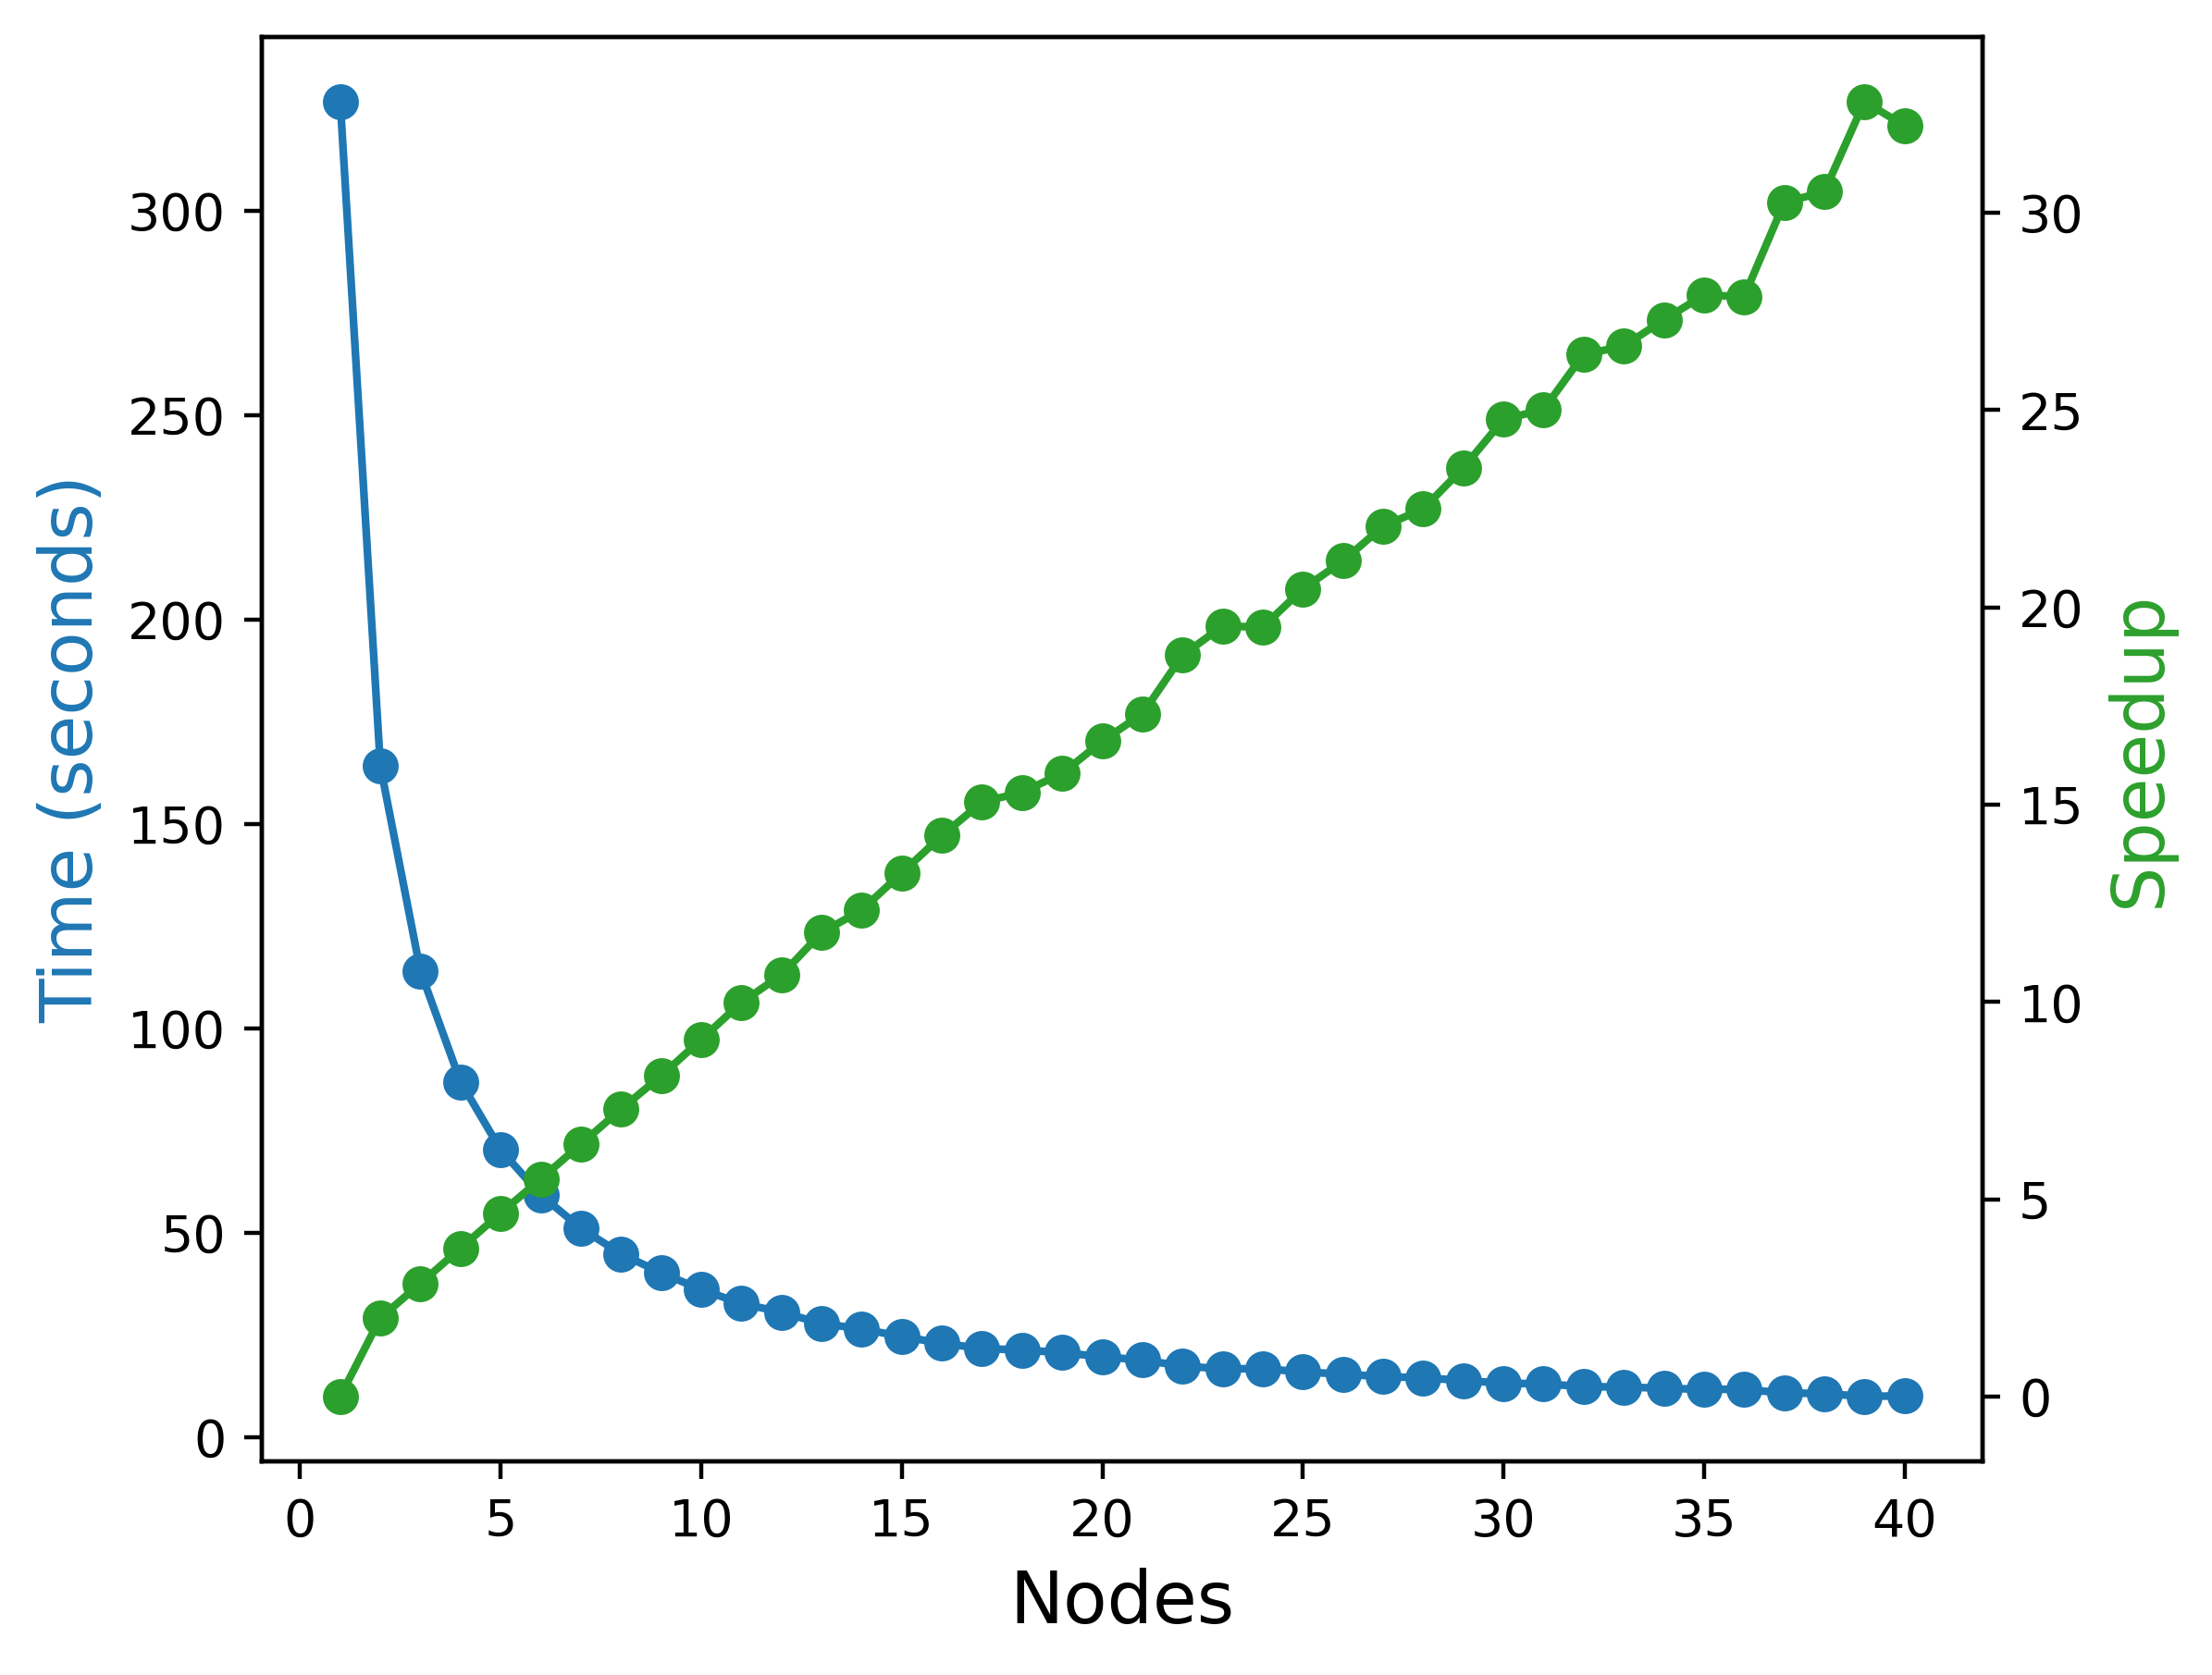
\includegraphics[width=\linewidth]{figs/mpi_strong.out}
	  \caption{Strong scaling analysis as MPI process count is increased}
      \Description{Speedup is nearly linear and time plateaus}
      \label{fig:mpi_strong}
    \end{minipage}
  \hspace{.05\linewidth}
 \begin{minipage}{0.45\linewidth}
  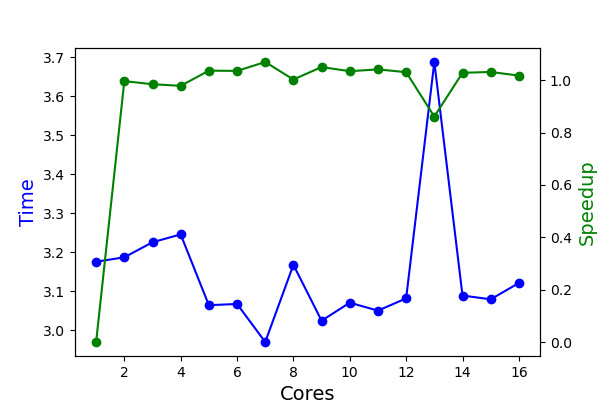
\includegraphics[width=\linewidth]{figs/omp_strong.out}
  \caption{Strong scaling analysis with OpenMP threads -- OpenMP is slightly faster}
    \Description{Weak scaling analysis relating mpi process count, time required for computation, and image width}
    \label{fig:omp_strong}
    \end{minipage}
\end{figure*}

All the results and analysis presented in this section were obtained
running our code on the Niagara supercomputer \cite{10.1145/3332186.3332195},
which is a large homogeneous cluster composed by 2,024 Lenovo SD530 servers
each with 40 Intel "Skylake"/"CascadeLake" cores working at approx. 2.4/2.5 GHz.
Each node of the cluster has 188 GiB/202 GB of RAM per node (at least 4 GiB/core for user jobs and roughly 170 GiB/node at most).
Being designed for large parallel workloads, it has a fast interconnect consisting of EDR InfiniBand in a Dragonfly+ topology with Adaptive Routing.


The first two figures, ~\ref{fig:mpi_weak2} and ~\ref{fig:omp_weak2} show a weak scaling analysis where we linearly increase the number of pixels rendered (starting at a 303 by 170 pixel image up to a 1920 by 1080 pixel image) and the single-node cores utilized in tandem. We observe that both OpenMP and MPI start at around 145 seconds, and increase logarithmically before plateauing roughly around 170-185 seconds per run. While ideally, we would observe a consistent time which does not increase, these results show relatively stable performance. We also witness OpenMP slightly outperforming MPI, which is expected, since MPI requires copying pixel data between processes. 

We witness something similar with the strong scaling results in figures ~\ref{fig:mpi_strong},~\ref{fig:omp_strong}. These results were run by increasing the number of cores used with a fixed workload. These results show an almost perfect convergence down to the serial fraction with similarly competitive results between OpenMP and MPI. In this case though, MPI slightly outperforms OpenMP as we approach 40 cores, with MPI's time converging to around 10 seconds, and openmp's time converging to around 11.


\begin{figure}[h]
  \centering
  \begin{minipage}{0.45\linewidth}
  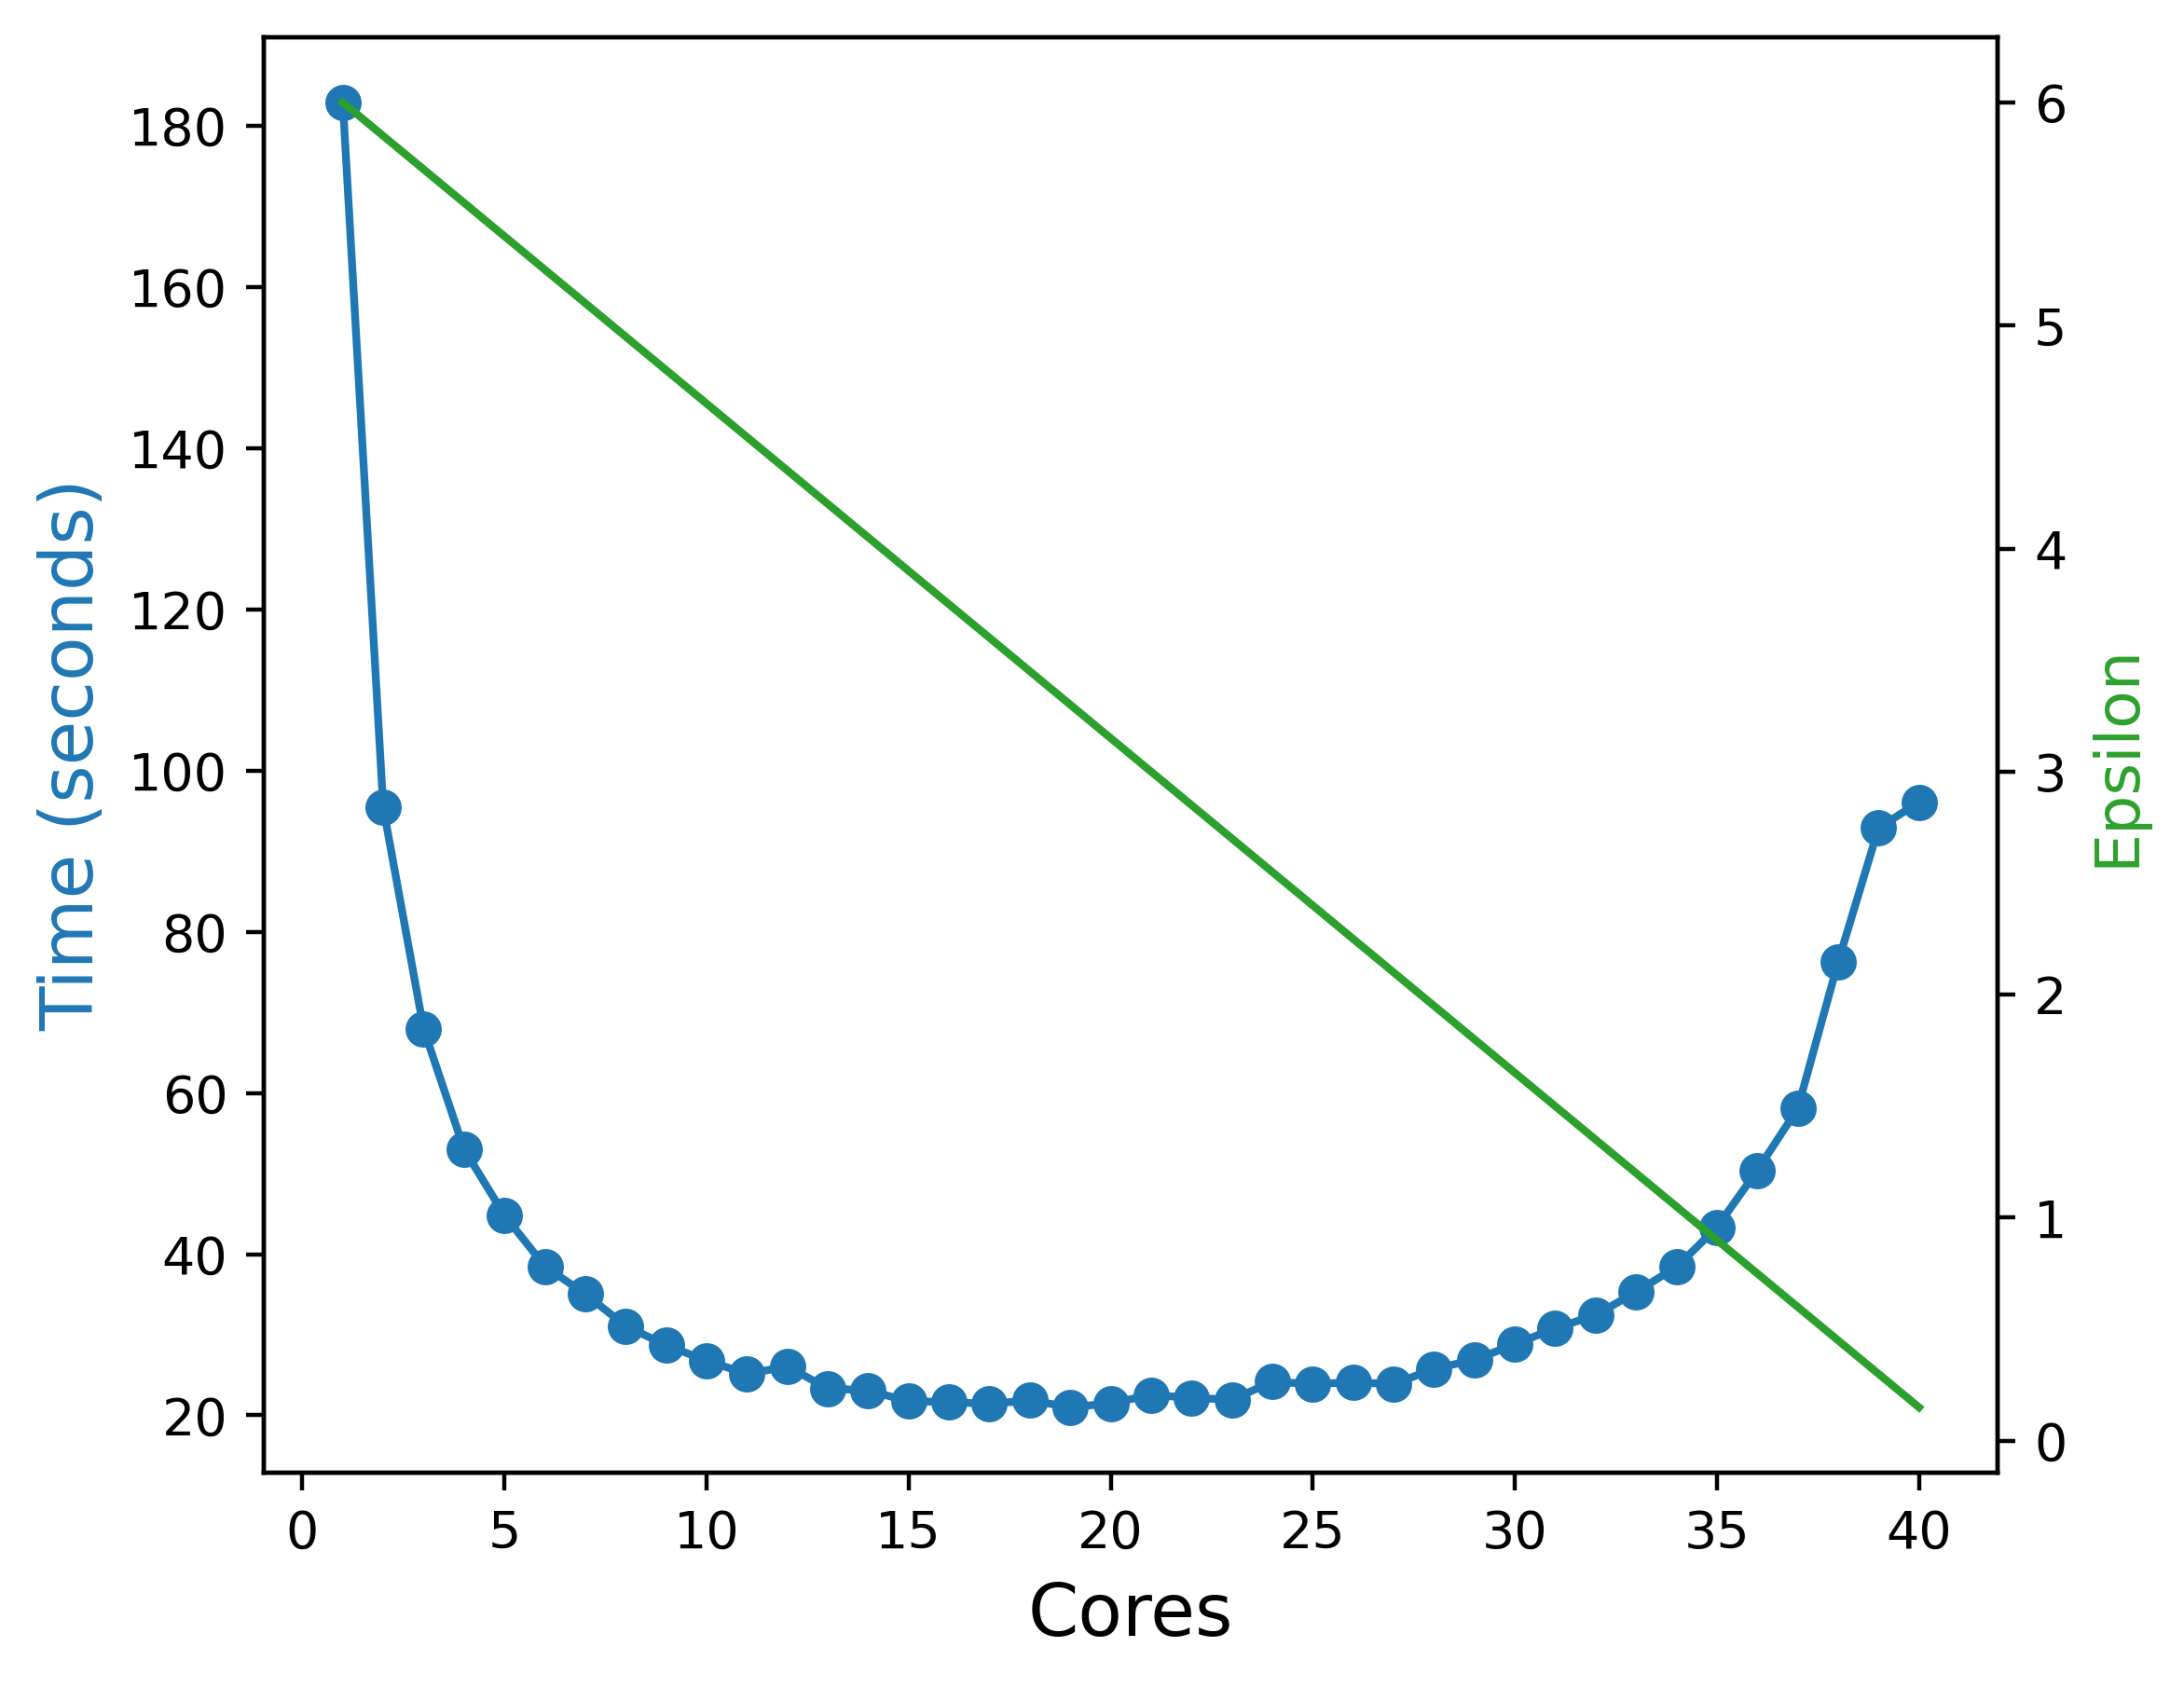
\includegraphics[width=\linewidth]{figs/omp_weak.out}
	\caption{Weak scaling analysis -- OMP thread count is increased and $\varepsilon$ is decreased in tandem}
    \Description{Weak scaling analysis relating OMP thread count, time required for computation, and $\varepsilon$ value.}
    \label{fig:omp_weak}
  \end{minipage}
  \hspace{.05\linewidth}
 \begin{minipage}{0.45\linewidth}
  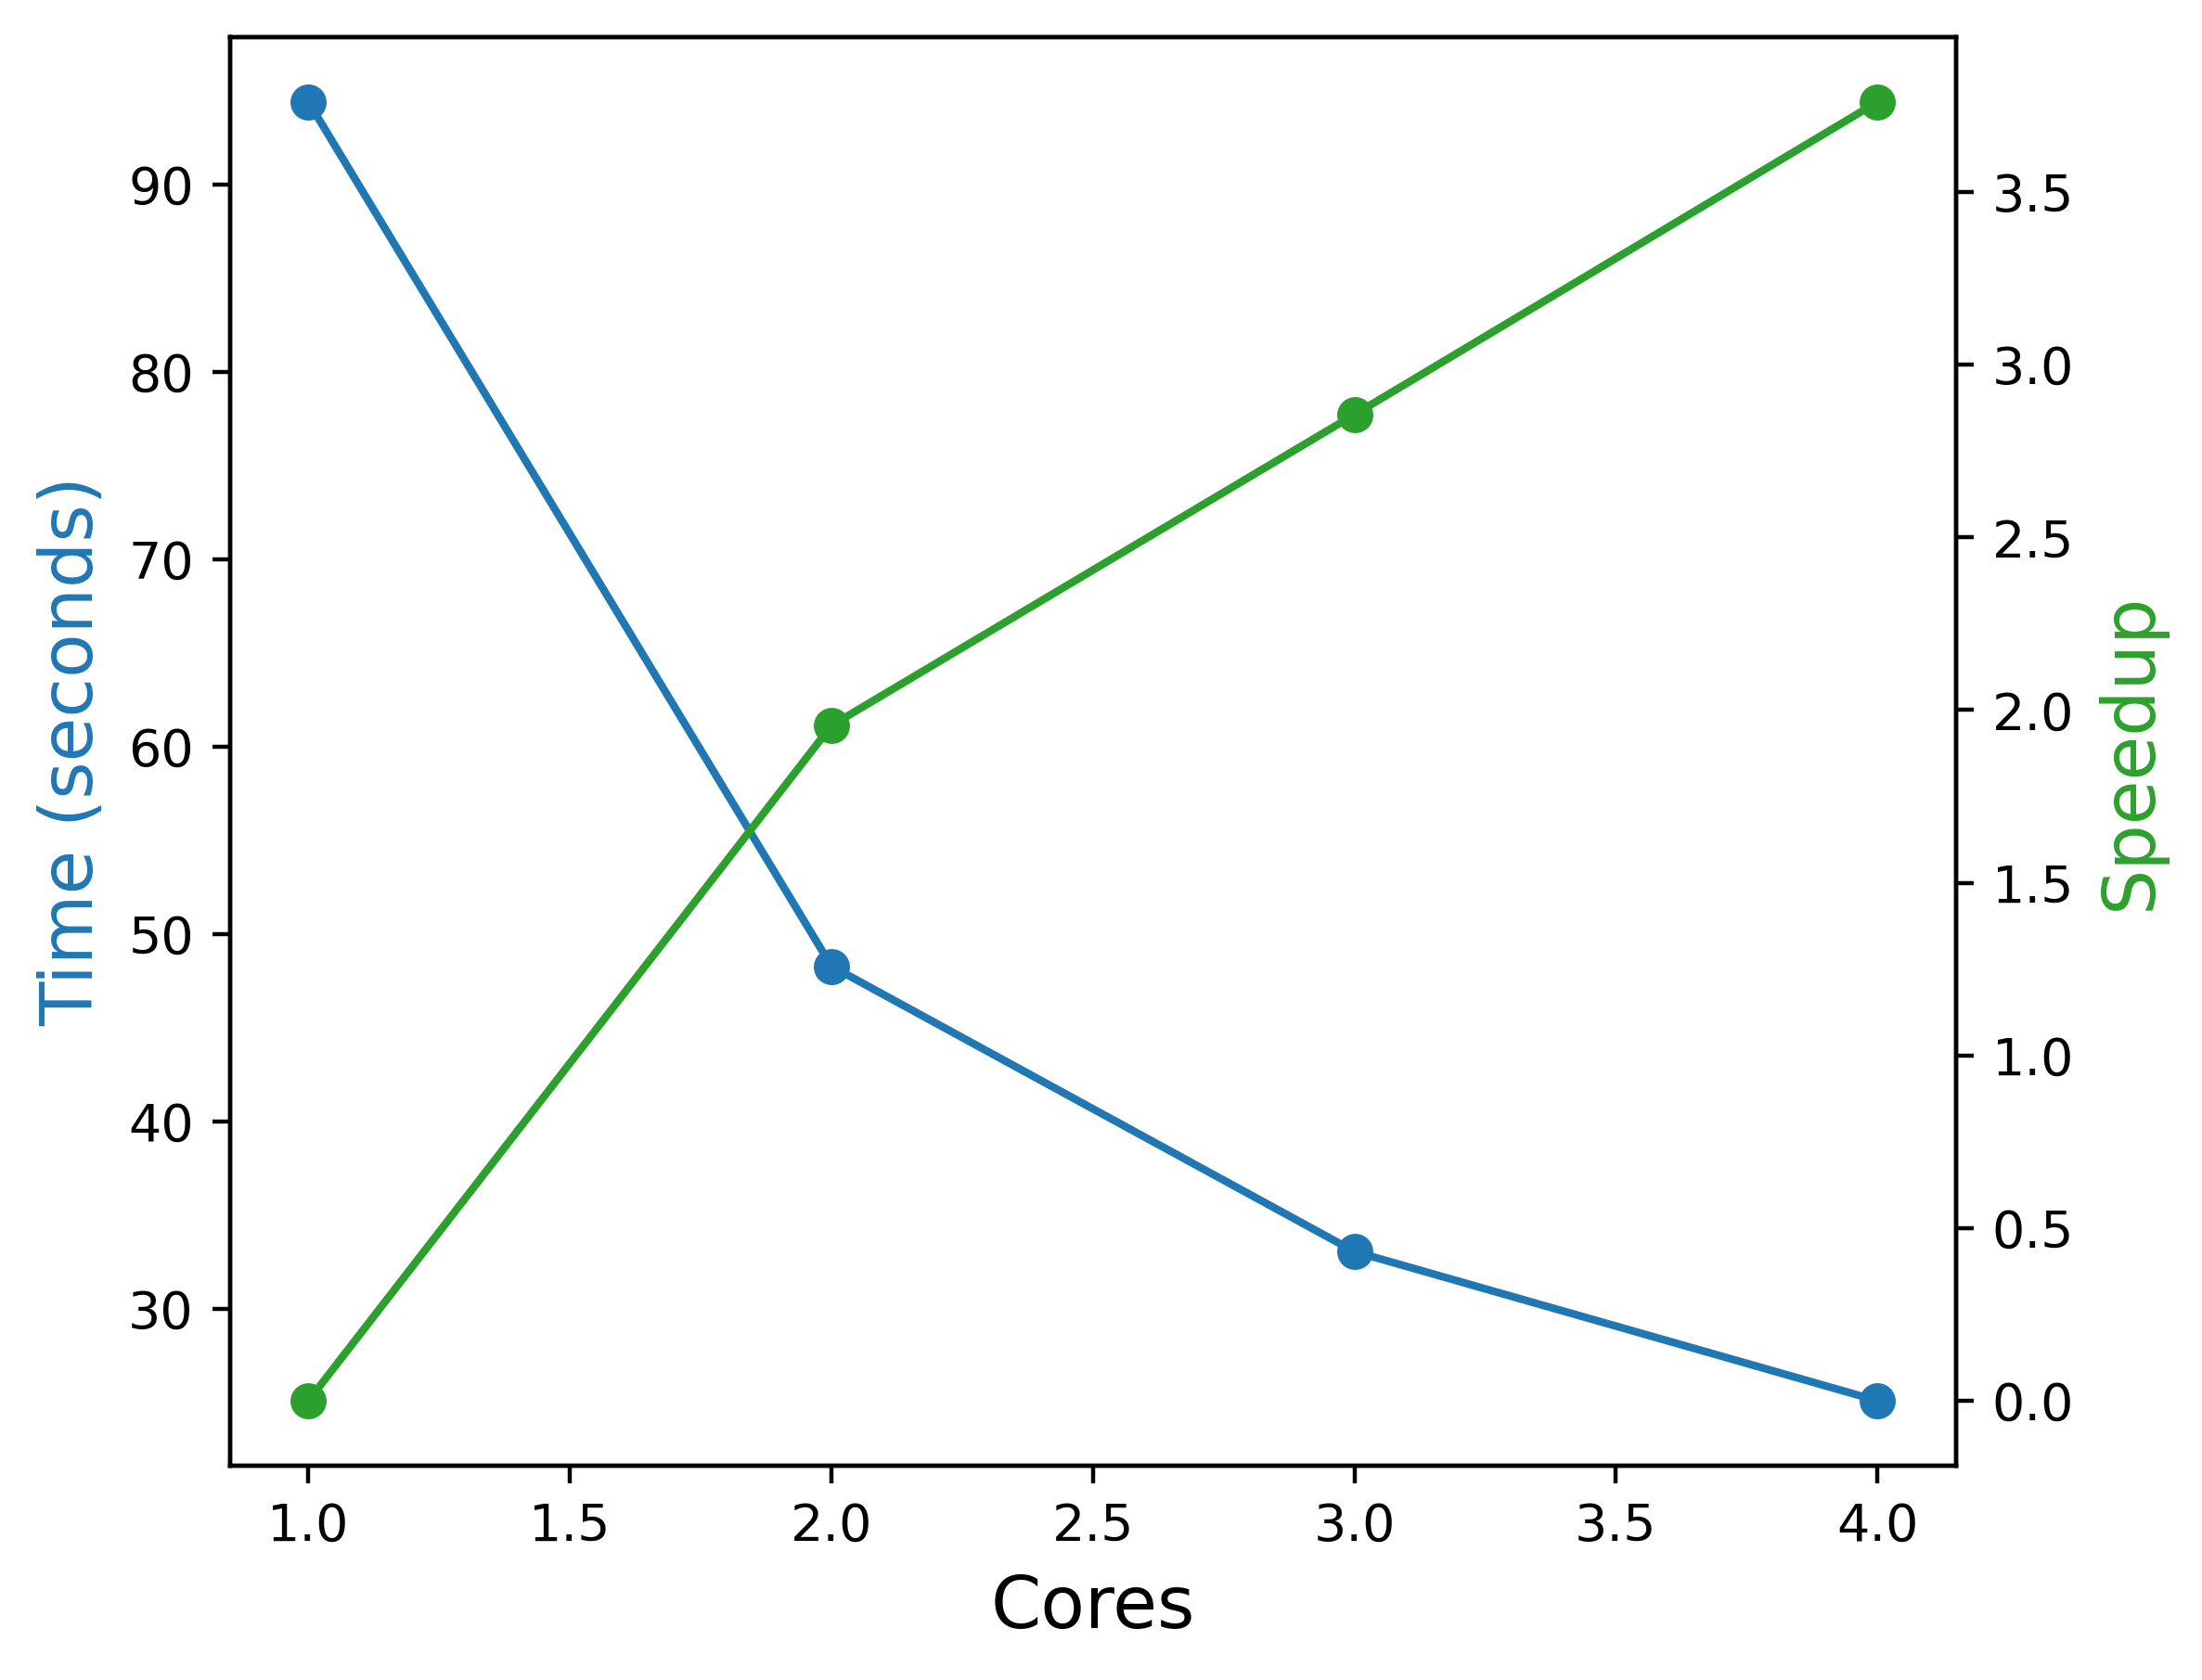
\includegraphics[width=\linewidth]{figs/mpi_strong_multinode.out}
  \caption{Multi-node run with 4 omp threads per node}
    \Description{Weak scaling analysis relating mpi process count, time required for computation, and image width}
    \label{fig:mpi_strong_multinode}
    \end{minipage}
\end{figure}

From Figure ~\ref{fig:omp_weak}, we can observe an abnormal scaling result. This run was taken by increasing the number of OpenMP threads utilized, while decreasing the simulation $\varepsilon$. We could be observing two phenomena here. For one, we could be witnessing some kind of contention which is not a factor in the 1-25 core range, but which degrades performance after 25 cores. Alternatively we could be witnessing an optimal value of $\varepsilon$, which dominates the performance gain from adding more cores. Because the results from the previous section show good scaling well into the 40 core range, both for weak and strong scaling, it is unlikely that we are observing exponential performance degradation, meaning it is more probable that we have found an optimal $\varepsilon$ value, which is somewhere around 4-2. 

Finally, from Figure ~\ref{fig:mpi_strong_multinode} we see a multi-node run with hybrid utilization of OpenMP and MPI. We set the OpenMP thread count to 4 cores, and scaled the number of nodes between 1 and 4. Notably, these results are quite similar to the single-node scaling runs. At 1 node (4 cores), we complete the job in 94 seconds, with single-node omp completing the run in 84 seconds. At 16 cores across 4 nodes, we complete the task in 25 seconds, with single-node OpenMP requiring 22 seconds. This shows that the Niagara cluster's interconnect is able to keep up with our application's network utilization. 


\CMT{M:Remind me: any comments or test on a hybrid, i.e. MPI+OMP approach? If not we can mention it as something to try in the discussion section, L: I added a run for this... limited to 4 nodes because of the trillium upgrades}


%%%%%%%%%%%%%%%%%%%%%%%%%%%%%%%%%%%%%%%%%%%%%%%%%%%%%%%%%%%%%%%%%%%%%


\section{Discussion}
\label{sec:disc}

\subsection{Educational Value}

This ray tracer implementation was originally developed as a final project for
an upper year specialized topics course in Computer Science, where the main
elements in the course were the discussion of High-Performance Computing
techniques.
As a rich computational project, it combines elments from mutliple disciplines, specifically
physics simulations (both through the use of a ray tracer, and through the simulation of gravitational distortion),
solutions to differential equational via approximations with GSL,
path stenciling, image/file parsing,
parallel and distributed computing with MPI and OpenMP, and domain decomposition,
as well as providing a bountiful quantity of variant implementations,
while being of relatively low-enough difficulty to be completed in a few weeks.
Moreover, it has the added value of being a 
program which is able to render realistic images.
In particular, the project would provide potential students an excellent opportunity to learn the practical use of GSL/ODE approximation in a realistic context.

The impact is felt in 3 areas:

1. Attempting to set up this particular system is theoretically easy and practically quite difficult. The initial conditions are not obvious. GSL asks for an initial radius, initial angle, and the derivative of the radius with respect to azimuthal angle. Unfortunately, it is not possible to find this derivative without an equation that models the trajectory of light rays, which is the equation we were trying to approximate in the first place! Solving this chicken-and-egg problem is a great educational experience, and forces one to consider more deeply the significance of the parameters given to GSL. 

2. Using GSL for course analysis is a nonstandard application. One key detail of the project is that we need to restrict the number of points GSL returns, while keeping the distance between points relatively even. The way this challenge was solved was by approximating the angle between the black hole on a line of potential future points, as described earlier, and having the GSL driver stencil the equation until it reaches said line. This also requires a more careful understanding of how GSL functions, and provides excellent learning outcomes.

3. The problem of relating the 2D ray-trajectory equation to a 3D scene has no readily available solutions. As such, it challenges potential students to think deeply about the problem, and to come up with original solutions.

Beyond the challenges associated with GSL, this project's requirement of parallel image processing provides an opportunity to learn how to process, parse, and generate large images in parallel. In particular, if one chooses to handle the case where the total handled image size is larger than system memory, then many variant implementations with considerable performance differences and technical complexity can be generated. 

Finally, this project provides an opportunity to practice domain decomposition techniques in a practical setting. Splitting and dividing work in the way domain decomposition requires is not often encountered in typical Computer Science education, so it is beneficial to provide more examples.


\subsection{General Applicability}
One interesting aspect of this design is it's general applicability. Variations of this technique can be used to render any sort of image under light distortion specified by a differential equation. In effect, any distortion function could be input into the ray tracer, and an image modeled under that distortion could be output. In the same line, this technique could be used to render images under the Kerr metric.


\subsection{Performance Tuning}
There is plenty of room for optimization on top of this ray tracer. A good place to start is that we could get away with calling into GSL significantly fewer times. When the light ray is far from the black hole, we can assume that the distortion is near zero, and thus, that we can simply compute the ray trajectory using Euclidean geometry. With certain settings, approximately 50\% of the ray tracer's runtime is spent inside GSL. Most of this time could be eliminated, resulting in much better performance. 


Another aspect of this implementation worth highlighting is its tight bottom-up parallel integration.
both in shared-memory and distributed-memory parallelism. Such implementation
allows for well-integrated and optimized scaling to run the ray tracer in larger problems.
This is a substantially more solid and potentially better scalable solution than other ones
where \textit{farm rendering} approaches are used \cite{10.1145/3528223.3530171,app112412046}.
Moreover the latter approaches would be only useful in cases of \textit{embarassignly parallel}
tasks (e.g. by splitting images or partioning independent data/field-views),
and even in those case it would be questionable whether or not the preparation work done required in 
order to prepare, administrate, and recombine these results is worth the cost.
Of course, we should not forget implementations employing \textit{GPU rendering}, for which
these devices and implementations are the most well-suited to be used \cite{Peddie2019_hardware}.
But as argued at the beginning of this work, those would be considered specialized devices
and even the corresponding implementations are tailored and fine-tuned to the specific hardware,
the benefit of which is best-in-class performance and scaling.


%%%%%%%%%%%%%%%%%%%%%%%%%%%%%%%%%%%%%%%%%%%%%%%%%%%%%%%%%%%%%%%%%%%%%

\section{Conclusions}
\label{sec:concl}

Gravitational lensing is a beautiful phenomenon, both when witnessed from space, and when digitally rendered. This paper explored a relatively simple method for creating a ray traced image which shows gravitational lensing, and how to accelerate the process using shared and distributed memory computing. Additionally, these types of projects lend themselves well to teaching and education, both with regards to general scientific computing techniques, and to HPC techniques.


%%%%%%%%%%%%%%%%%%%%%%%%%%%%%%%%%%%%%%%%%%%%%%%%%%%%%%%%%%%%%%%%%%%%%
